\chapter{從粒子到簡單量子場}

讓我們再從稍有不同的角度，建構這個簡單的量子場。進入量子場論有兩條路：我們可以從粒子出發，探究為什麼場是描述粒子的自然語言；也可以從波場出發，探究為什麼它的激發以量子的形式出現。兩條路都很有用。這裡我們走第一條。

普通量子力學可以描述一個粒子、兩個粒子，或任何其他固定粒子數。自然界並不受這項限制。每當燈發射或吸收輻射，房間裡的光子數就會改變。不穩定粒子會衰變。例如在 {\proseunicodefont β} 衰變中，
\begin{equation}
n\longrightarrow p+e^-+\bar{\nu}_e,
\end{equation}
因此，數種粒子的數量會同時改變。我們需要一套足夠廣泛的量子力學，能容納所有可能的佔據數，並且最終能描述佔據數彼此轉換的過程。

目前我們先大幅簡化問題：只有一種非相對論性粒子。我們先擴大它的態空間，使其能容納任意粒子數，之後再討論更多粒子種類、相對論、散射與衰變。數學本身並不特別困難，但觀點的轉變很抽象。值得放慢腳步，免得記號掩蓋了想法。

\section{從單粒子出發}

先從一個處於態 \(|\psi\rangle\) 的單粒子開始。它在位置空間中的波函數為
\begin{equation}
\psi(x)=\langle x|\psi\rangle.
\label{eq:l07-wavefunction}
\end{equation}
這個小寫的 \(\psi\) 是普通的複值函數。它還不是量子場，也不是作用於多粒子態空間的算符。

玻恩定則指出，
\begin{equation}
\rho_\psi(x)=|\psi(x)|^2=\psi^*(x)\psi(x)
\label{eq:l07-born-density}
\end{equation}
是粒子出現在 \(x\) 處的機率密度。對於歸一化的態，
\begin{equation}
\int dx\,\psi^*(x)\psi(x)=1.
\label{eq:l07-one-particle-normalization}
\end{equation}
右側等於總機率。由於這裡恰好只有一個粒子，總機率也恰好等於粒子數。這個巧合雖然在此無足為奇，稍後卻會成為有用的線索。

\begin{classroomqa}
\lecturetimestamp{00:09:13}
\audiencequestion{為什麼機率密度必須寫成 \(\psi^*(x)\psi(x)\) 的形式？}
\lecturerresponse{這就是玻恩定則，是量子力學的公設之一。位置測量結果為 \(x\) 的振幅是 \(\langle x|\psi\rangle\)；機率密度則是振幅的絕對值平方。這不是從後文的場構造推導出來的。}
\end{classroomqa}

\section{模式、正交性與完備性}

單粒子希爾伯特空間有許多有用的基底。位置本徵態構成一組基底；任何厄米算符的本徵態也構成另一組基底，但簡併與連續譜的情況須按通常方式處理。由於能量很快就會派上用場，我們選取一組完備且正交歸一的單粒子能量本徵態：
\begin{equation}
|1\rangle,\ |2\rangle,\ldots,
\qquad
\psi_i(x)=\langle x|i\rangle.
\end{equation}

盒中粒子的例子讓指標 \(i\) 變得具體。基態波函數沒有內部節點，下一個態有一個節點，更高能態的振盪則愈來愈快。對理想的無限深方形位能井而言，這些波函數本質上就是正弦波。

\begin{figure}[htbp]
\centering
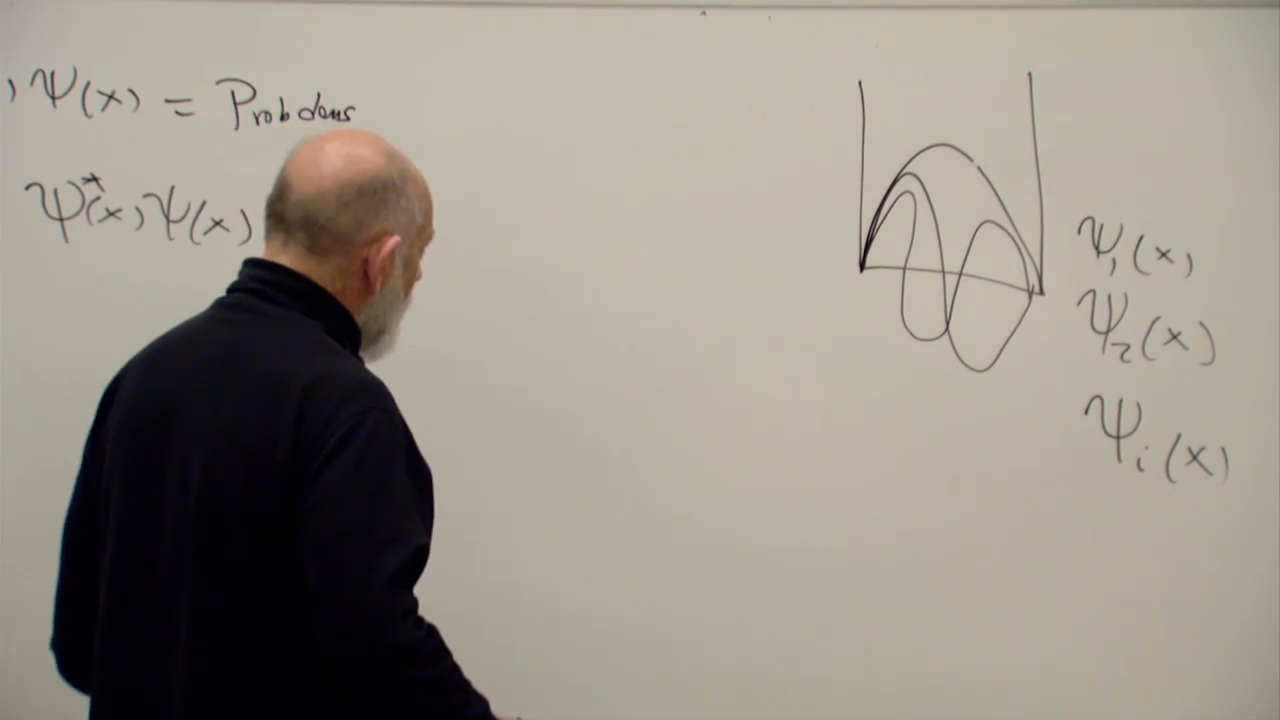
\includegraphics[width=0.94\linewidth]{lecture_07_frame_01.png}
\caption{課堂黑板上的盒中模式。左側殘留的內容是單粒子的玻恩機率密度與歸一化；右側的位能井則畫出 \(\psi_1(x)\)、\(\psi_2(x)\)，以及一般標記 \(\psi_i(x)\)。}
\lectureframe{00:08:25}
\end{figure}

即使黑板上的內容有所遮擋，仍可分辨出相同的模式結構：
\begin{figure}[htbp]
\centering
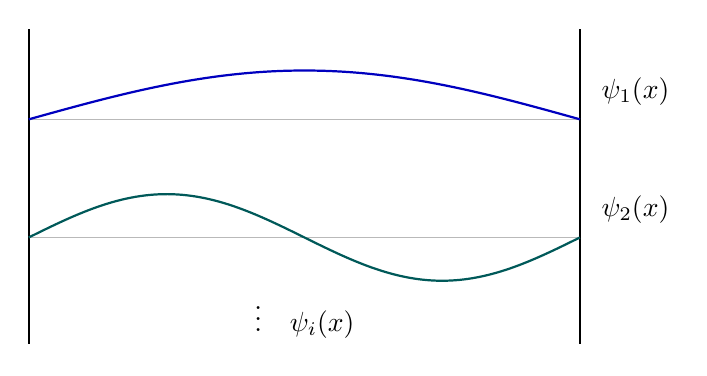
\begin{tikzpicture}[x=1cm,y=1cm]
  \draw[thick] (0,0) -- (0,4.0);
  \draw[thick] (7,0) -- (7,4.0);
  \draw[gray!55] (0,2.85) -- (7,2.85);
  \draw[gray!55] (0,1.35) -- (7,1.35);
  \draw[blue!75!black,thick,domain=0:7,samples=120]
    plot (\x,{2.85+0.62*sin(180*\x/7)});
  \draw[teal!70!black,thick,domain=0:7,samples=120]
    plot (\x,{1.35+0.55*sin(360*\x/7)});
  \node[right] at (7.15,3.20) {$\psi_1(x)$};
  \node[right] at (7.15,1.70) {$\psi_2(x)$};
  \node at (3.5,0.38) {$\vdots\quad\psi_i(x)$};
\end{tikzpicture}
\caption{盒中模式示意圖的清晰重繪。兩個波函數在垂直方向上的位移只是為了方便展示。}
\end{figure}

正交歸一關係為
\begin{equation}
\int dx\,\psi_i^*(x)\psi_j(x)=\delta_{ij}.
\label{eq:l07-orthonormality}
\end{equation}
若 \(i=j\)，態便已歸一化，積分值為一；若 \(i\ne j\)，兩個態便彼此正交，積分值為零。

同樣重要的完備性關係是
\begin{equation}
\sum_i |i\rangle\langle i|=\mathbf 1.
\label{eq:l07-resolution}
\end{equation}
每個 \(|i\rangle\langle i|\) 都投影到一個基底方向；對完備基底求和則得到恆等算符。它作用於任意向量時，只是先將向量分解成各分量，再將分量合併還原。

現在將式~\eqref{eq:l07-resolution}夾在兩個位置態之間：
\begin{align}
\langle y|x\rangle
&=\sum_i\langle y|i\rangle\langle i|x\rangle \\
&=\sum_i\psi_i(y)\psi_i^*(x) \\
&=\delta(y-x).
\label{eq:l07-position-completeness}
\end{align}
複共軛星號應加在左矢右矢順序為 \(\langle i|x\rangle\) 的那一項上。交換 \(x\) 和 \(y\) 的位置，便會得到複共軛但等價的形式。因此，每一組完備的正交歸一基底都能表示 {\proseunicodefont δ} 函數。正弦函數、餘弦函數、振子波函數與能量本徵函數都能完成同樣的工作。

\begin{classroomqa}
\lecturetimestamp{00:13:43}
\audiencequestion{完備性求和中的第二個波函數是否應該帶有複共軛？}
\lecturerresponse{是的。依照 \(\langle y|i\rangle\langle i|x\rangle\) 的順序，兩個因子是 \(\psi_i(y)\psi_i^*(x)\)。保留明確的左矢右矢順序，就不必靠猜測來決定星號的位置，也能避免放錯。}
\end{classroomqa}

這就是我們需要的單粒子數學。現在來改變態空間。

\section{作為擴大態空間的福克空間}

對許多全同粒子而言，一組方便的基底會記錄每個單粒子模式中有多少粒子：
\begin{equation}
|n_1,n_2,n_3,\ldots\rangle.
\label{eq:l07-fock-basis}
\end{equation}
整數 \(n_i\) 是模式 \(i\) 的佔據數。這個右矢不是用花俏記號寫成的單粒子態；它屬於一個更大的希爾伯特空間，其中包含零粒子扇區、所有單粒子態、所有雙粒子態，依此類推。這個更大的空間稱為福克空間。

若要改變佔據數，便為每個模式引入一個產生算符和一個湮滅算符：
\begin{equation}
a_i^\dagger,\qquad a_i.
\end{equation}
前者在模式 \(i\) 中增加一個粒子，後者則移除一個粒子。在這裡，諧振子的語言只是記錄佔據數的工具：不一定真有一根彈簧在振動。諧振子代數恰好提供了升高與降低佔據數所需的機制。

模式數算符為
\begin{equation}
\begin{aligned}
N_i&=a_i^\dagger a_i,\\
N_i|n_1,\ldots,n_i,\ldots\rangle
&=n_i|n_1,\ldots,n_i,\ldots\rangle.
\end{aligned}
\end{equation}
真空態為
\begin{equation}
|0\rangle\equiv|0,0,0,\ldots\rangle,
\qquad
a_i|0\rangle=0
\quad\text{for every }i.
\label{eq:l07-vacuum}
\end{equation}
因此，模式 \(i\) 中的單粒子態為
\begin{equation}
|i\rangle=a_i^\dagger|0\rangle.
\label{eq:l07-mode-created}
\end{equation}
同一個符號 \(|i\rangle\) 現在既可以表示單粒子基底向量，也可以表示嵌入福克空間單粒子扇區中的該向量。這項嵌入由式~\eqref{eq:l07-mode-created}給出；我們正在討論哪個空間，則由上下文決定。

\section{將各模式組合成場}

定義湮滅場與產生場如下：
\begin{equation}
\Psi(x)=\sum_i \psi_i(x)a_i,
\qquad
\Psi^\dagger(x)=\sum_i \psi_i^*(x)a_i^\dagger.
\label{eq:l07-field-expansion}
\end{equation}
大小寫很重要。小寫函數 \(\psi_i(x)\) 是複數；大寫的 \(\Psi(x)\) 則是作用於福克空間的算符。對每個空間位置 \(x\)，式~\eqref{eq:l07-field-expansion}都給出一個不同的模式算符線性組合。這就是「位置的算符值函數」的意思。

對自由粒子，模式函數可以是平面波 \(e^{ikx}\)。此時式~\eqref{eq:l07-field-expansion}便是傅立葉展開，只是傅立葉係數由算符而非數值構成。舊有術語把普通複數稱為 \(c\) 數，把量子算符稱為 \(q\) 數。模式函數是 \(c\) 數，與所有對象都對易；\(a_i\) 和 \(a_i^\dagger\) 則具有算符的性質。

\(\Psi\) 和 \(\Psi^\dagger\) 都不是厄米算符；它們的厄米共軛互為對方。以下兩個組合
\begin{equation}
\Psi+\Psi^\dagger,
\qquad
i(\Psi^\dagger-\Psi)
\label{eq:l07-hermitian-combinations}
\end{equation}
則是厄米算符，可以代表可觀測量。不過目前而言，場最有用之處，是能在局部產生、湮滅並計數粒子。

\begin{classroomqa}
\lecturetimestamp{00:21:05}
\audiencequestion{算符依賴於 \(x\) 是什麼意思？}
\lecturerresponse{意思是，\(x\) 的每個取值都對應一個不同的算符。空間依賴性來自普通的模式函數，而每個由此得到的線性組合都作用於同一個福克空間。}
\end{classroomqa}

\section{產生場的作用}

要知道定義有何用處，就得看它如何作用。從單粒子扇區中的位置本徵態出發，並插入單位算符的完備關係：
\begin{align}
|x\rangle
&=\sum_i |i\rangle\langle i|x\rangle \\
&=\sum_i a_i^\dagger|0\rangle\,\psi_i^*(x) \\
&=\Psi^\dagger(x)|0\rangle.
\label{eq:l07-local-creation}
\end{align}
因此，\(a_i^\dagger\)會在確定的模式 \(i\) 中產生一個粒子；\(\Psi^\dagger(x)\)則會在位置 \(x\) 產生一個局域化的粒子。在理想化的位置基底中，這種局域化是以分布的意義成立；實際製備會使用狹窄的波包，但代數上的意義相同。

\begin{classroomqa}
\lecturetimestamp{00:24:48}
\audiencequestion{\(\sum_i|i\rangle\langle i|\)是投影算符嗎？}
\lecturerresponse{每一項都是投影到一個基底態的投影算符。對完整基底求和得到的就是恆等算符，稱為單位算符的完備關係。插入這個關係不會改變任何態，卻能顯示該態在所選基底中的各個分量。}
\end{classroomqa}

式~\eqref{eq:l07-local-creation}直接揭示了場的粒子意義。我們不只是替抽象算符加上空間標記，而是構造出在該空間位置產生粒子的操作。

\begin{classroomqa}
\lecturetimestamp{00:28:20}
\audiencequestion{位置空間中的產生場應該標上星號還是匕首？}
\lecturerresponse{算符的厄米共軛要用匕首符號。星號表示普通波函數 \(\psi_i(x)\) 的複共軛；匕首符號則標在 \(a_i^\dagger\) 和 \(\Psi^\dagger(x)\) 上。}
\end{classroomqa}

\begin{classroomqa}
\lecturetimestamp{00:28:36}
\audiencequestion{在模式展開式中，可以把產生算符移過波函數嗎？}
\lecturerresponse{可以。\(\psi_i(x)\) 是 \(c\) 數，因此與所有算符都對易。只有在調換 \(a_i\) 和 \(a_j^\dagger\) 這類不對易算符的順序時，才需要小心。}
\end{classroomqa}

\section{從機率密度到粒子密度}

現在來看看這個場。首先自然會考慮
\begin{equation}
\int dx\,\Psi^\dagger(x)\Psi(x).
\end{equation}
它看起來像單粒子的歸一化積分，但現在其中的因子是算符。代入模式展開式，並保持算符的順序不變：
\begin{align}
\int dx\,\Psi^\dagger(x)\Psi(x)
&=\int dx
\left(\sum_i a_i^\dagger\psi_i^*(x)\right)\\
&\qquad\times\left(\sum_j a_j\psi_j(x)\right) \\
&=\sum_{i,j}a_i^\dagger a_j
\int dx\,\psi_i^*(x)\psi_j(x) \\
&=\sum_{i,j}a_i^\dagger a_j\,\delta_{ij} \\
&=\sum_i a_i^\dagger a_i.
\label{eq:l07-number-derivation}
\end{align}
因此，總粒子數算符為
\begin{equation}
N=\sum_i N_i
=\int dx\,\Psi^\dagger(x)\Psi(x).
\label{eq:l07-total-number}
\end{equation}
對於這裡討論的態，高能模式上的佔據數會逐漸趨近於零，因此即使可能的模式無窮多，粒子總數通常仍有限。

被積分項是局部粒子密度算符：
\begin{equation}
n(x)=\Psi^\dagger(x)\Psi(x).
\label{eq:l07-density}
\end{equation}
嚴格來說，密度不能在數學上的單一點測量。對於小區域 \(R\)，實際測量的是
\begin{equation}
N_R=\int_R dx\,n(x),
\label{eq:l07-regional-number}
\end{equation}
也就是該區域內的粒子數。和其他量子可觀測量一樣，\(N_R\) 在任意態中不一定有確定值。重複製備同一狀態，測量結果可能不同。

\begin{classroomqa}
\lecturetimestamp{00:36:27}
\audiencequestion{\(\Psi^\dagger(x)\Psi(x)\)是多粒子機率密度嗎？}
\lecturerresponse{它直接表示的是粒子密度。多粒子機率振幅一般取決於所有粒子的座標；而這個局部雙線性算符若在某個小區域上積分，計算的則是該區域內的粒子數。}
\end{classroomqa}

\begin{classroomqa}
\lecturetimestamp{00:38:28}
\audiencequestion{算符 \(a_i\) 和 \(a_i^\dagger\) 只作用於態向量，不作用於單粒子波函數嗎？}
\lecturerresponse{是的。它們作用於福克空間中的態，例如 \(|n_1,n_2,\ldots\rangle\)。乘在這些算符前面的單粒子模式函數是普通數值，並非這些升降算符作用的對象。}
\end{classroomqa}

佔據數態構成一組基底，卻不是一般態的唯一形式。它們可以疊加；例如，總粒子數相同，但粒子在不同模式間分布方式不同的態也可以疊加。對光子這類中性粒子而言，不同總粒子數的態也可以疊加。式~\eqref{eq:l07-regional-number}中的算符在這些態中都具有相同的操作意義。

\begin{classroomqa}
\lecturetimestamp{00:40:01}
\audiencequestion{若以總粒子數除粒子密度，是否就得到粒子出現在 \(x\) 處的機率密度？}
\lecturerresponse{在固定 \(N\) 且粒子數很大的情況下，\(N_R/N\) 是相對頻率，通常能很好地反映單粒子機率。但這並不是一條算符恆等式，不能把單次測量結果等同於機率。在獨立粒子的圖像中，測得的計數會有漲落，典型幅度約為 \(\sqrt N\)；偶爾一次測量也可能與機率相差很大，雖然這種情況不常見。}
\end{classroomqa}

\begin{classroomqa}
\lecturetimestamp{00:42:25}
\audiencequestion{若將一電子態與零電子態疊加，電荷守恆會如何？}
\lecturerresponse{這不是固定電荷封閉扇區中所使用的那種疊加。可以疊加總電荷相同、但粒子分布不同的態。光子不帶電，因此不同光子數扇區的疊加不會造成這個問題。電子數與正電子數也可以同時改變，而淨電荷仍保持不變。}
\end{classroomqa}

\section{獨立粒子的能量}

接下來要看的是能量。先考慮彼此不交互作用的粒子。在稀薄系統中，這通常是很好的近似。原則上，光子也會透過高階過程彼此交互作用；但普通實驗室中的輻射足夠稀薄，因此獨立粒子的描述非常準確。

令 \(\omega_i\) 表示模式 \(i\) 中單一粒子的能量，其中 \(\hbar=1\)。模式就是一個單粒子態。於是總哈密頓量為
\begin{equation}
H=\sum_i\omega_i N_i
=\sum_i\omega_i a_i^\dagger a_i.
\label{eq:l07-mode-hamiltonian}
\end{equation}
每個被佔據的模式中，每一個粒子都各自貢獻一次其單粒子能量。

\begin{classroomqa}
\lecturetimestamp{00:48:16}
\audiencequestion{\(\omega_i\)是位置的函數嗎？}
\lecturerresponse{不是。它是與模式 \(i\) 對應的能量本徵值。函數 \(\psi_i(x)\) 依賴位置；\(\omega_i\) 則取決於選中了哪個能階。}
\end{classroomqa}

數值 \(\omega_i\) 由單粒子定態薛丁格方程決定。定義
\begin{equation}
h=-\frac{\nabla^2}{2m}+V(x).
\label{eq:l07-one-particle-h}
\end{equation}
於是
\begin{equation}
h\psi_i(x)=\omega_i\psi_i(x).
\label{eq:l07-schrodinger-eigenvalue}
\end{equation}
在一維中，動量算符是 \(p=-i\partial_x\)，而 \(p^2/(2m)\) 就是 \(-\partial_x^2/(2m)\)。在三維中，三個二階導數合併為 \(-\nabla^2/(2m)\)。

\begin{figure}[htbp]
\centering
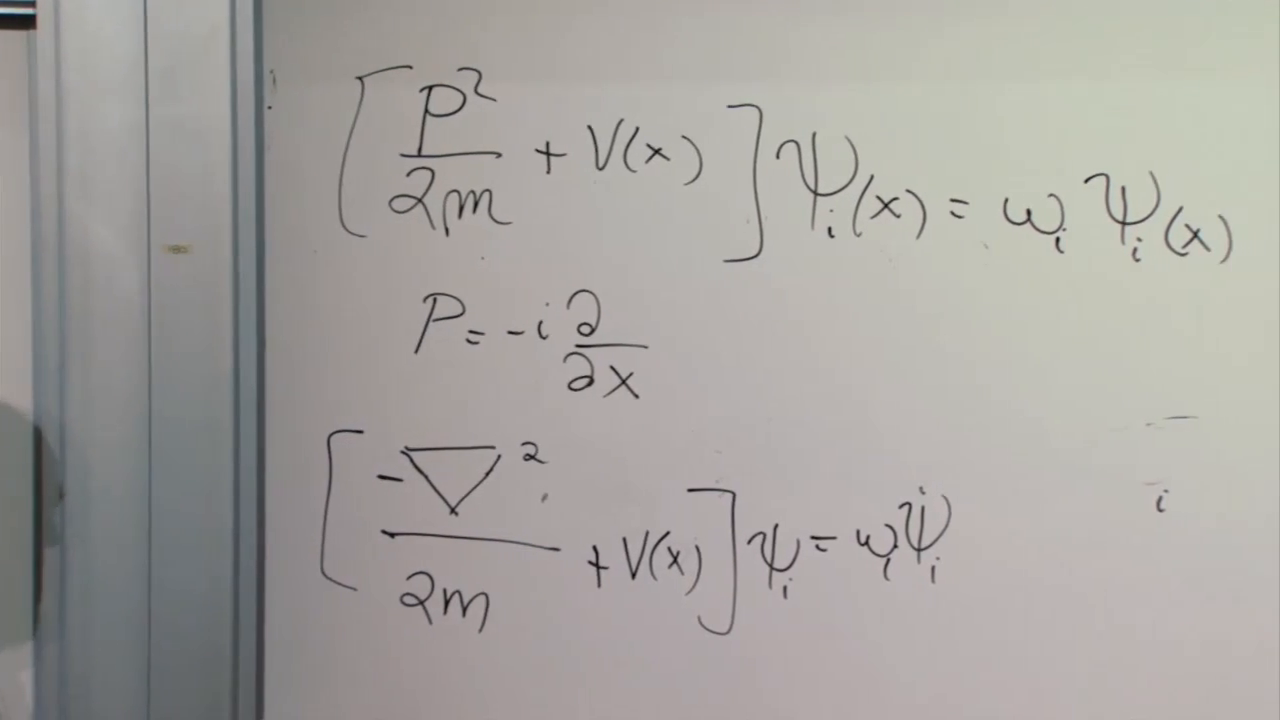
\includegraphics[width=0.94\linewidth]{lecture_07_frame_02.png}
\caption{黑板上從 \(p^2/(2m)+V(x)\) 推到單粒子薛丁格本徵值方程微分形式的過程。式~\eqref{eq:l07-schrodinger-eigenvalue}是整理後的重構版本。}
\lectureframe{00:54:10}
\end{figure}

對任意歸一化的單粒子波函數，熟知的能量期望值為
\begin{equation}
\langle h\rangle_\psi
=\int dx\,\psi^*(x)h\psi(x).
\label{eq:l07-one-particle-energy-expectation}
\end{equation}
多粒子公式可以從這個形式得到提示：把小寫的波函數換成算符值場。這還不是證明，而是我們接下來要檢驗的猜想：
\begin{equation}
H=\int dx\,\Psi^\dagger(x)h\Psi(x).
\label{eq:l07-field-hamiltonian}
\end{equation}

\section{先寫出答案，再加以證明}

將式~\eqref{eq:l07-field-expansion}代入所提出的哈密頓量：
\begin{align}
\int dx\,\Psi^\dagger h\Psi
&=\int dx
\left(\sum_i a_i^\dagger\psi_i^*(x)\right)
h\left(\sum_j a_j\psi_j(x)\right) \\
&=\sum_{i,j}a_i^\dagger a_j
\int dx\,\psi_i^*(x)h\psi_j(x).
\label{eq:l07-h-expanded}
\end{align}
微分算符 \(h\) 作用於依賴 \(x\) 的波函數 \(\psi_j(x)\)，而不是作用於模式算符 \(a_j\)。根據薛丁格方程，
\begin{equation}
h\psi_j(x)=\omega_j\psi_j(x).
\end{equation}
因此，
\begin{align}
\int dx\,\Psi^\dagger h\Psi
&=\sum_{i,j}a_i^\dagger a_j\omega_j
\int dx\,\psi_i^*(x)\psi_j(x) \\
&=\sum_{i,j}a_i^\dagger a_j\omega_j\delta_{ij} \\
&=\sum_j\omega_j a_j^\dagger a_j.
\label{eq:l07-h-proof}
\end{align}
這正是式~\eqref{eq:l07-mode-hamiltonian}。局部場的表示式與所有粒子能量的總和，是同一個算符。

\begin{figure}[htbp]
\centering
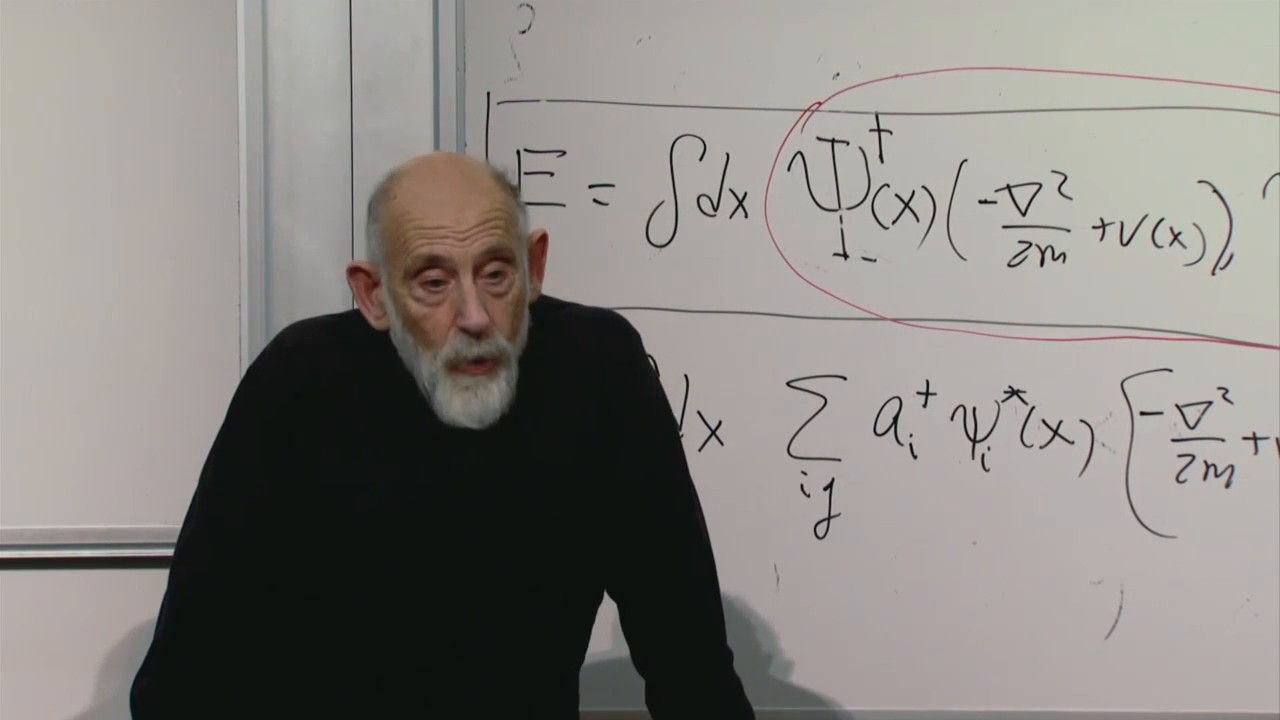
\includegraphics[width=0.94\linewidth]{lecture_07_frame_03.png}
\caption{黑板上著重標示的場哈密頓量，下方則開始以模式展開式進行證明。保留課堂畫面作為佐證；式~\eqref{eq:l07-field-hamiltonian}--\eqref{eq:l07-h-proof}補上完整的推導。}
\lectureframe{01:05:34}
\end{figure}

這段推導中，沒有把任何產生算符移過湮滅算符。\(a_i^\dagger a_j\) 的順序從頭到尾都保持不變。只有 \(c\) 數波函數及其本徵值可以任意移動。

\section{為什麼稱它為場}

為什麼稱 \(\Psi(x)\) 為場？因為它是在空間每一點定義的算符值量，而由它構成的厄米組合或雙線性算符則是局部可觀測量。密度 \(n(x)\) 與下文的局部能量表示式就是兩個例子。「場」這個詞背後沒有其他隱藏的數學判準。

這個場不是電磁場，而是描述提供單粒子模式與哈密頓量 \(p^2/(2m)+V\) 的非相對論性粒子種類，例如緩慢運動的原子、中子、質子或電子。這些粒子是各自對應場的量子；就結構而言，這與光子是電磁場的量子相同。

\begin{classroomqa}
\lecturetimestamp{01:02:45}
\audiencequestion{從多粒子系統推到上述公式時，場是在哪一步引入的？}
\lecturerresponse{場是在式~\eqref{eq:l07-field-expansion}引入的：\(\Psi(x)\)在每個空間位置都是一個算符。後續推導顯示，它的局部乘積可以測量粒子密度與能量密度。具有空間依賴性且包含算符，正是我們正在建構的場結構。}
\end{classroomqa}

\section{局部能量密度}

式~\eqref{eq:l07-field-hamiltonian}將總能量寫成空間積分：
\begin{equation}
\begin{aligned}
H&=\int dx\,\mathcal H(x),\\
\mathcal H(x)
&=-\frac{1}{2m}\Psi^\dagger(x)\nabla^2\Psi(x)\\
&\quad+V(x)\Psi^\dagger(x)\Psi(x).
\end{aligned}
\label{eq:l07-hamiltonian-density}
\end{equation}
被積項是這個哈密頓量自然的一種局部能量密度，但局部形式並不唯一。例如，分部積分可以把動能項改寫為
\begin{equation}
\mathcal H_{\rm kin}(x)
=\frac{1}{2m}\nabla\Psi^\dagger(x)\mathbin{\cdot}\nabla\Psi(x)
\label{eq:l07-kinetic-density}
\end{equation}
兩者只差一個邊界項。在通常的邊界條件下，這兩種表示式給出相同的總哈密頓量。這就是課堂上提到的那點不唯一性。

\begin{classroomqa}
\lecturetimestamp{01:05:57}
\audiencequestion{能量密度一定要在全空間積分嗎？}
\lecturerresponse{在全空間積分會得到總能量；在較小區域積分，則得到歸屬於該區域的能量。這仍受局部密度選取方式不唯一的影響，只要對全空間積分後得到相同的哈密頓量即可。}
\end{classroomqa}

\begin{classroomqa}
\lecturetimestamp{01:06:25}
\audiencequestion{能量公式中的大寫 \(N_i\) 與小寫 \(n_i\) 有何不同？}
\lecturerresponse{\(N_i=a_i^\dagger a_i\)是算符。整數 \(n_i\) 則是它在佔據數態上的其中一個本徵值。算符作用於態；本徵值則是普通數值。}
\end{classroomqa}

\begin{classroomqa}
\lecturetimestamp{01:06:46}
\audiencequestion{能否用狄拉克符號把場哈密頓量本身寫成左矢或右矢？}
\lecturerresponse{不能。左矢與右矢表示態向量及其對偶；場與哈密頓量則是作用於這些態的算符。像 \(\langle\Phi|H|\Phi\rangle\) 這樣的期望值同時涉及兩類對象，不應將兩者混為一談。}
\end{classroomqa}

\section{重現單粒子理論，並邁向經典場}

擴大的形式架構包含了普通的單粒子量子力學。將福克空間限制在滿足下式的態：
\begin{equation}
N|\Phi\rangle=|\Phi\rangle.
\end{equation}
在這個扇區中，場的構造會重現所有單粒子態與單粒子預測。我們並未取代舊理論，而是把它嵌入一個也能描述零個、兩個或任意多個粒子的空間中。

在另一個極端，若某個模式中有大量玻色子，它就可能近似呈現經典波的行為。在適當的相干態或半經典態中，期望值
\begin{equation}
\Phi_{\rm cl}(x,t)=\langle\Psi(x,t)\rangle
\end{equation}
對自由非相對論性理論滿足下列看似經典的方程：
\begin{equation}
i\partial_t\Phi_{\rm cl}(x,t)
=\left(-\frac{\nabla^2}{2m}+V(x)\right)\Phi_{\rm cl}(x,t)
\label{eq:l07-classical-schrodinger}
\end{equation}
課堂上指出這項關聯，但沒有加以推導。這是量子粒子集合與波場之間的橋梁：大量佔據會抑制相對漲落，使適當的期望值呈現經典行為。

因此，這套形式架構既是記帳工具，也是物理描述。它整理了所有粒子數扇區，也刻畫干涉、糾纏，以及經典波如何從量子粒子中浮現。

\begin{classroomqa}
\lecturetimestamp{01:10:43}
\audiencequestion{為什麼在積分中操作產生與湮滅算符時，幾乎可以把它們當成普通數值？}
\lecturerresponse{它們彼此從未交換順序。普通模式函數與這些算符對易，而導數只作用於那些函數。若要把湮滅算符移過產生算符，就必須使用對易子，也可能因此多出一項；但證明中的任何一步都沒有進行這種操作。}
\end{classroomqa}

\section{狄拉克符號小插曲}

有些混淆源自歷史背景。單粒子波函數滿足波動方程，表面上看似經典場，同時卻又是機率振幅。早期量子理論必須先區分這兩種角色，再說明電磁學這類真正可測量的波場如何由量子構成。福克空間與算符值場化解了這個表面上的矛盾。

狄拉克符號能以極精簡的方式呈現這種區別。右矢屬於向量空間，左矢屬於其對偶空間，兩者並置便構成內積。有了完備關係
\begin{equation}
\sum_i|i\rangle\langle i|=\mathbf 1
\end{equation}
整個過程幾乎一目了然。課堂上用一則向數學家講授量子力學的軼事說明這一點：數學內容原本就熟悉，但符號讓常見運算變得如此清楚，整體結構看起來竟像是新發現。重點不是哪個學科缺少這個概念，而是恰當的符號能讓合法的運算不易混淆。

這個道理在此很重要。現在有幾種不同的算符：
\begin{itemize}
\item \(h\) 作為微分算符作用於單粒子波函數；
\item \(a_i\) 和 \(a_i^\dagger\) 作用於福克空間中的佔據數態；
\item \(\Psi(x)\)、\(\Psi^\dagger(x)\)、\(N\) 與 \(H\) 也作用於福克空間。
\end{itemize}
式~\eqref{eq:l07-field-expansion}中的展開式連結了前兩種情境，但沒有把它們混為一談。

\begin{classroomqa}
\lecturetimestamp{01:18:16}
\audiencequestion{場只是描述粒子集合的一套形式架構嗎？}
\lecturerresponse{場論確實是一套形式架構，但並非空洞的形式。場的局部可觀測量可以測量；粒子則是具有干涉與糾纏的量子粒子，而非經典小球。場算符恰好編碼了這些可測量的集體性質。}
\end{classroomqa}

\section{相對論的提醒與電磁學旁論}

目前的構造是非相對論性的。在相對論物理中，動量仍是良好的粒子標記，但要嚴格局域化粒子位置則複雜得多。因此，局部光子數密度通常不像非相對論性的 \(n(x)\) 那樣明確。能量密度仍有良好定義，是較可靠的局部可觀測量。

課堂上提出一個有用、但明確僅供啟發的電磁類比。將電場與磁場組合成複向量：
\begin{equation}
\mathbf F=\mathbf E+i\mathbf B,
\qquad
\mathbf F^*=\mathbf E-i\mathbf B.
\label{eq:l07-riemann-silberstein}
\end{equation}
於是
\begin{equation}
\mathbf F^*\mathbin{\cdot}\mathbf F
=\mathbf E^2+\mathbf B^2,
\label{eq:l07-em-density}
\end{equation}
在慣用單位制下，它與電磁能量密度成正比。這並不是真正的光子機率密度。較恰當的看法是：它是能以模平方表示能量密度的精簡場變數；非正式地說，也可把它理解為以光子能量加權的光子密度。

\begin{classroomqa}
\lecturetimestamp{01:19:10}
\audiencequestion{光子密度能否等同於電場強度？}
\lecturerresponse{只能在定性層次上謹慎地這麼說。對相對論性光子而言，局部粒子數不是首選概念。可靠的說法是，\(E^2+B^2\) 與能量密度成正比，而複數組合 \(\mathbf E+i\mathbf B\) 則將馬克士威方程組寫成類似薛丁格方程的形式。}
\end{classroomqa}

\begin{classroomqa}
\lecturetimestamp{01:20:09}
\audiencequestion{為什麼相對論性粒子可以有確定動量，位置卻成問題？}
\lecturerresponse{動量能清楚標記相對論性單粒子表示；嚴格局域化則與粒子產生及相對論性場描述相牴觸。本講不會進一步發展這套理論；此處的提醒是要指出，目前非相對論性密度詮釋的適用界限。}
\end{classroomqa}

\section{算符排序與基態常數}

不能任意改變算符的順序。對玻色模式而言，
\begin{equation}
a_i a_i^\dagger=a_i^\dagger a_i+1.
\end{equation}
因此，將正規排序的 \(\Psi^\dagger h\Psi\) 改成反向排序的 \((h\Psi)\Psi^\dagger\)，或改成適當積分後的對應形式，都會多出對易子項。在模式基底中，這是一個對每個模式各加上一個能量量子的總和。這就是基態常數，也稱零點能常數；在連續情況下，還需要對它進行調節。本講不會進一步探討這個問題，只提醒兩種排序並不相等。

\begin{classroomqa}
\lecturetimestamp{01:22:04}
\audiencequestion{如果在哈密頓量中交換 \(\Psi\) 與 \(\Psi^\dagger\) 的順序，會發生什麼事？}
\lecturerresponse{必須計入它們的對易子。因此，顛倒順序會多出一項與態無關的基態貢獻，而不會得到相同的表示式。展示的哈密頓量採用正規序，\(\Psi^\dagger h\Psi\)。}
\end{classroomqa}

\section{動量作為最後的檢驗}

最後幾分鐘再次進行相同的提升。對單一粒子而言，
\begin{equation}
\langle p\rangle_\psi
=\int dx\,\psi^*(x)\left(-i\partial_x\right)\psi(x).
\label{eq:l07-one-particle-momentum}
\end{equation}
將波函數換成場，即得到總動量算符
\begin{equation}
P=\int dx\,\Psi^\dagger(x)\left(-i\partial_x\right)\Psi(x),
\label{eq:l07-field-momentum}
\end{equation}
在三維中則為
\begin{equation}
\mathbf P=\int d^3x\,\Psi^\dagger(\mathbf x)
\left(-i\boldsymbol\nabla\right)\Psi(\mathbf x).
\end{equation}
場會攜帶動量。足夠強的雷射會將動量傳遞給牆壁，並對牆壁施力；在量子描述中，場的動量就是所有光子動量的總和。

式~\eqref{eq:l07-field-momentum}是算符，不是期望值。給定一個 Fock 空間中的態 \(|\Phi\rangle\)，便可以計算
\begin{equation}
\langle P\rangle_\Phi=\langle\Phi|P|\Phi\rangle.
\end{equation}
要形成期望值，算符和態缺一不可。若把可觀測量與其平均值混為一談，就會抹去本講一直努力建立的區分。

\begin{classroomqa}
\lecturetimestamp{01:26:02}
\audiencequestion{展示的場動量已經是平均動量了嗎？}
\lecturerresponse{不是。它是代表該可觀測量的厄米算符。給定一個態，將算符夾在該態的左矢與右矢之間，才能得到期望值；測量結果仍可能在平均值附近有所漲落。}
\end{classroomqa}

這裡是自然的收尾。從粒子出發，我們構造了局域的產生場與湮滅場，用它們計數粒子，並將單粒子能量與動量的總和改寫為場算符。下一步不再只是改變記號，而是讓場算符描述物理過程：粒子衰變、粒子散射，以及不同種類的粒子彼此轉化。
